\documentclass[tikz]{standalone}

\usepackage{mathtools}

\usetikzlibrary{positioning,arrows}


\begin{document}
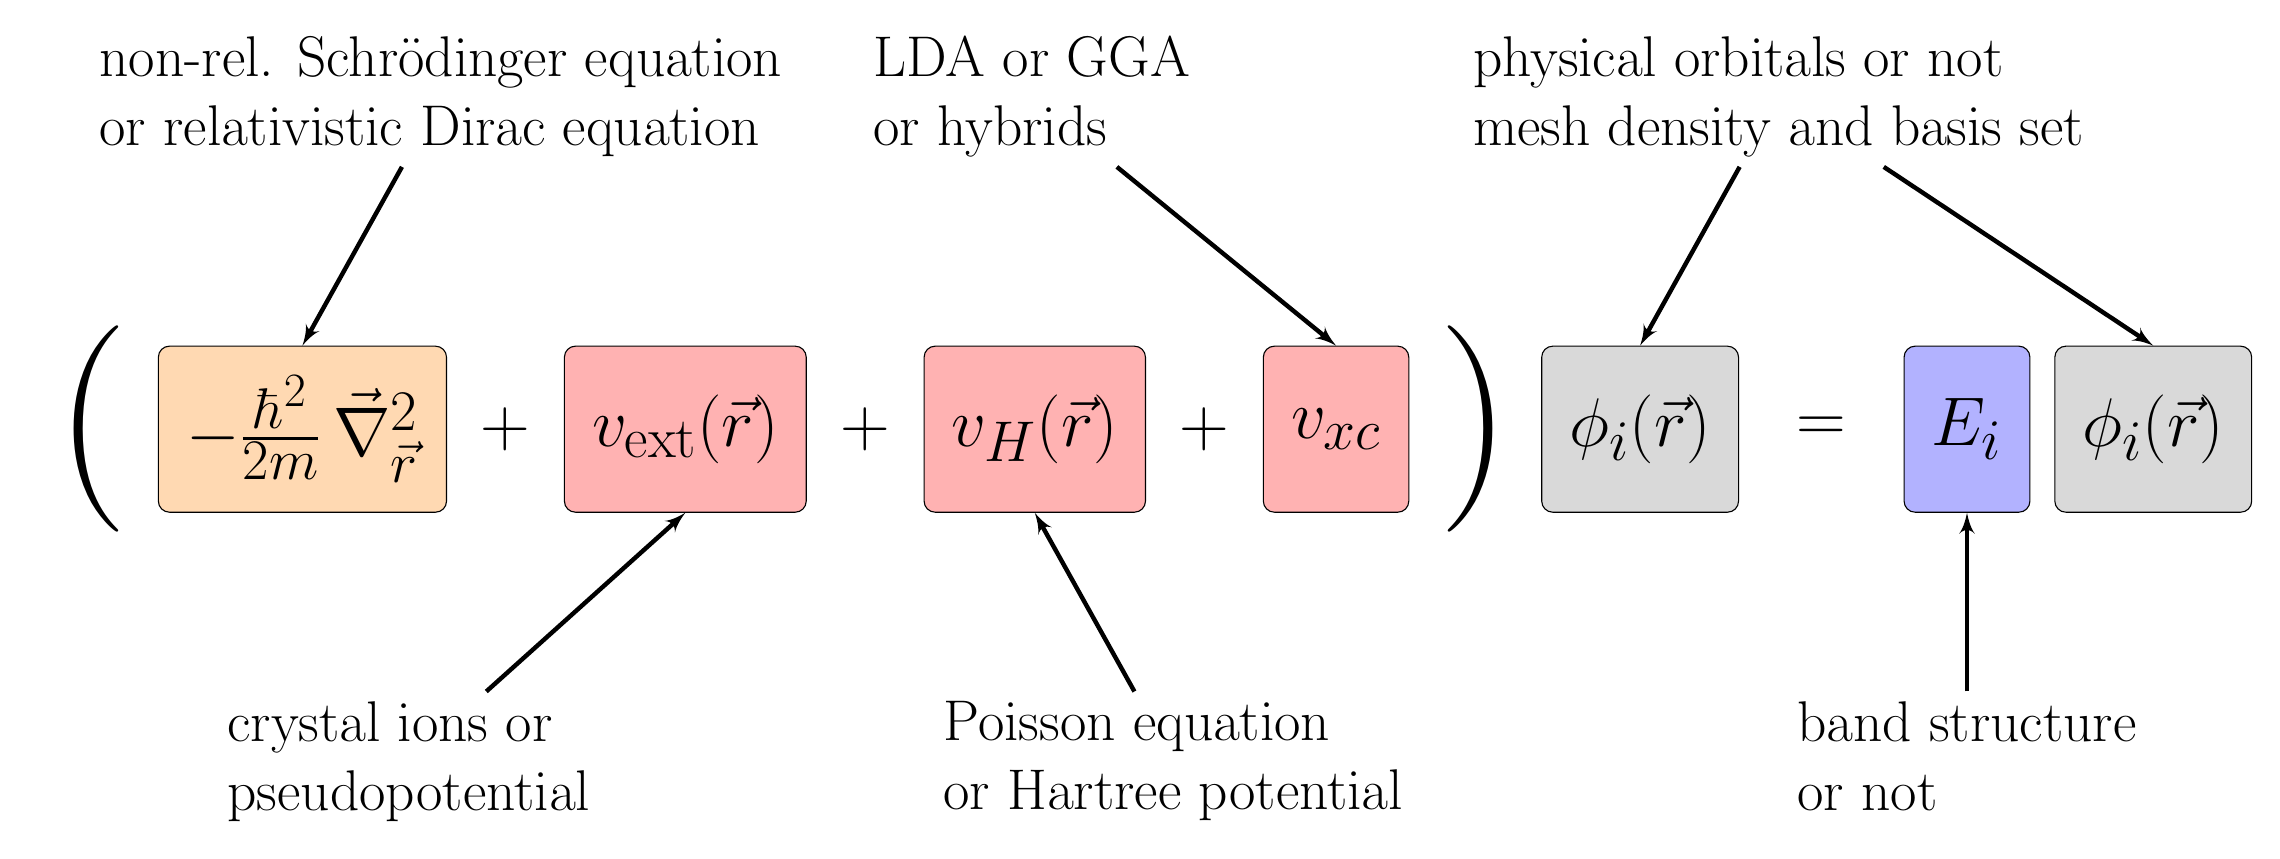
\begin{tikzpicture}[
    g/.style={rectangle,draw,rounded corners,minimum height=6em,inner sep=1em,font=\Huge},
    w/.style={font=\Huge},
    c/.style={node distance=15ex,align=left,font=\huge},
    a/.style={draw,-latex',ultra thick}
  ]

  \node [w,scale=3] (bra) {(};
  \node [node distance=0ex,fill=orange!30,g,right=of bra] (kinetic) {$-\frac{\hbar^2}{2m}\,\vec{\nabla}_{\vec{r}}^2$};
  \node [node distance=2ex,w,right=of kinetic] (plus1) {$+$};
  \node [node distance=2ex,fill=red!30,g,right=of plus1] (external) {$v_\text{ext}(\vec{r})$};
  \node [node distance=2ex,w,right=of external] (plus2) {$+$};
  \node [node distance=2ex,fill=red!30,g,right=of plus2] (hartree) {$v_H(\vec{r})$};
  \node [node distance=2ex,w,right=of hartree] (plus3) {$+$};
  \node [node distance=2ex,fill=red!30,g,right=of plus3] (xc) {$v_{xc}$};
  \node [node distance=0ex,w,right=of xc,scale=3] (ket) {)};
  \node [node distance=0ex,fill=gray!30,g,right=of ket] (phi1) {$\phi_i(\vec{r})$};
  \node [node distance=4ex,w,right=of phi1] (equal) {$=$};
  \node [node distance=4ex,fill=blue!30,g,right=of equal] (energy) {$E_i$};
  \node [node distance=2ex,fill=gray!30,g,right=of energy] (phi2) {$\phi_i(\vec{r})$};

  \node [c,above=of kinetic,xshift=5em] (kinetic comment) {non-rel. Schrödinger equation\\or relativistic Dirac equation};
  \node [c,below=of external,xshift=-10em] (external comment) {crystal ions or\\pseudopotential};
  \node [c,below=of hartree,xshift=5em] (hartree comment) {Poisson equation\\or Hartree potential};
  \node [c,above=of xc,xshift=-11em] (xc comment) {LDA or GGA\\or hybrids};
  \node [c,above=of phi1,xshift=5em] (phi comment) {physical orbitals or not\\mesh density and basis set};
  \node [c,below=of energy] (energy comment) {band structure\\ or not};

  \path [a] (kinetic comment) -- (kinetic.north);
  \path [a] (external comment) -- (external.south);
  \path [a] (hartree comment) -- (hartree.south);
  \path [a] (xc comment) -- (xc.north);
  \path [a] (phi comment) -- (phi1.north);
  \path [a] (phi comment) -- (phi2.north);
  \path [a] (energy comment) -- (energy.south);

\end{tikzpicture}
\end{document}